\documentclass[journal,12pt,twocolumn]{IEEEtran}

\usepackage{setspace}
\usepackage{gensymb}

\singlespacing


\usepackage[cmex10]{amsmath}
\usepackage{amsthm}
\usepackage{mathrsfs}
\usepackage{txfonts}
\usepackage{stfloats}
\usepackage{bm}
\usepackage{cite}
\usepackage{cases}
\usepackage{subfig}
\usepackage{longtable}
\usepackage{multirow}
\usepackage{mathtools}
\usepackage{steinmetz}
\usepackage{tikz}
\usepackage{circuitikz}
\usepackage{verbatim}
\usepackage{tfrupee}
\usepackage[breaklinks=true]{hyperref}
\usepackage{tkz-euclide} % loads  TikZ and tkz-base
%\usetkzobj{all}
\usetikzlibrary{calc,math}
\usepackage{listings}
    \usepackage{color}                                            %%
    \usepackage{array}                                            %%
    \usepackage{longtable}                                        %%
    \usepackage{calc}                                             %%
    \usepackage{multirow}                                         %%
    \usepackage{hhline}                                           %%
    \usepackage{ifthen}                                           %%
  %optionally (for landscape tables embedded in another document): %%
    \usepackage{lscape}     
\usepackage{multicol}
\usepackage{chngcntr}
\DeclareMathOperator*{\Res}{Res}
\renewcommand\thesection{\arabic{section}}
\renewcommand\thesubsection{\thesection.\arabic{subsection}}
\renewcommand\thesubsubsection{\thesubsection.\arabic{subsubsection}}

\renewcommand\thesectiondis{\arabic{section}}
\renewcommand\thesubsectiondis{\thesectiondis.\arabic{subsection}}
\renewcommand\thesubsubsectiondis{\thesubsectiondis.\arabic{subsubsection}}

\DeclarePairedDelimiter\abs{\lvert}{\rvert} % \abs{} for numerisk værdi
\DeclarePairedDelimiter\norm{\lVert}{\rVert}
\makeatletter
\let\oldabs\abs
\def\abs{\@ifstar{\oldabs}{\oldabs*}}
\let\oldnorm\norm
\def\norm{\@ifstar{\oldnorm}{\oldnorm*}}
\makeatother


\newcommand{\bignorm}[1]{\Bigl \| #1 \Bigr \| #1}
% correct bad hyphenation here
\hyphenation{op-tical net-works semi-conduc-tor}
\def\inputGnumericTable{}                                 %%

\lstset{
frame=single, 
breaklines=true,
columns=fullflexible
}


\begin{document}
\begin{center}
\huge Assignment 2\\

\large Matish Singh Tanwar\\
\large AI20MTECH11005\\
\end{center}
\vspace{1.0cm}
\begin{abstract}
This document finds the equation of a plane which is at a distance of 7 units from origin and normal to $\begin{pmatrix}3\\5\\6\end{pmatrix}$
\end{abstract}
\vspace{0.5cm}
Download all python codes from 
\begin{lstlisting}
https://github.com/Matish007/Matrix-Theory-EE5609-/tree/master/Assignment_2/codes
\end{lstlisting}
%
and latex-tikz codes from 
\begin{lstlisting}
https://github.com/Matish007/Matrix-Theory-EE5609-/tree/master/Assignment_2
\end{lstlisting}
%
\vspace{0.5mm}
\section{Problem}
Find the equation of a plane which is at a distance of 7 units from origin and normal to $\begin{pmatrix}3\\5\\6\end{pmatrix}$\\
\begin{align}
    \mathbf{n}=\begin{pmatrix}3\\5\\6\end{pmatrix}
\end{align}
\section{Explanation}
Let the equation of plane be:-\\
\begin{align}
   \mathbf{n}^T\mathbf{x} = c
\end{align}
where $\mathbf{n}$=normal vector to the plane\\
The distance from the origin is given by:-
\begin{align}
    \frac{\abs{c}}{\norm{\mathbf{n}}} = 7\\
    \norm{\mathbf{n}}=\sqrt{3^2+5^2+6^2}=\sqrt{70}
\end{align}\\
Substituting equation (4) in (3) we get,
\begin{align}
    \frac{\abs{c}}{\sqrt{70}}=7\\
    c=\pm{7\sqrt{70}}
\end{align}\\
Substituting equation (1),(6) in (2) we get two equation of planes,
\begin{align}
    \boxed{\begin{pmatrix}3 & 5 & 6\end{pmatrix}\mathbf{x}=7\sqrt{70}}\\
     \boxed{\begin{pmatrix}3 & 5 & 6\end{pmatrix}\mathbf{x}=-7\sqrt{70}}
\end{align}
Equation (7) and (8) gives us the equation of two planes which are at a distance of 7 units from origin and normal to $\begin{pmatrix}3\\5\\6\end{pmatrix}$
\begin{figure}[h!]
	\centering
	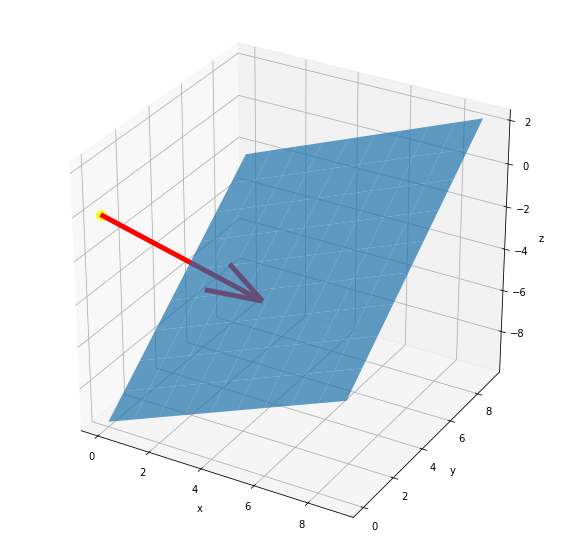
\includegraphics[width=\columnwidth]{plane.png}
	\caption{Planes with Normal vectors}
	\label{myfig}
\end{figure}
\end{document}
